\documentclass[10pt]{beamer}
\usepackage[utf8]{inputenc}
%\usepackage[dvipsnames]{xcolor}
\usepackage{charter}
\usepackage{amsmath}
\usepackage{amsfonts}
\usepackage{mathtools}
\usepackage{amssymb}
\usepackage{hyperref}
\usepackage[ruled,vlined]{algorithm2e}
\usepackage{commath}

\newcommand\pro{\item[\textbf{+}]}
\newcommand\con{\item[\textbf{--\kern 1.2pt}]}

% justify text in bibliography
\usepackage{ragged2e}  % for \justifying
\usepackage{etoolbox}
\apptocmd{\thebibliography}{\justifying}{}{}
\usepackage{natbib} 
\bibliographystyle{plainnat}
% links in blue
\definecolor{links}{HTML}{2A1B81}
\hypersetup{colorlinks=true,citecolor=blue,linkcolor=,urlcolor=links}


\title{Stochastic variance reduced gradient methods \\for training Deep Neural Networks}
\author{Alexander Apostolov}
\institute {École Polytechnique Fédérale de Lausanne}
\date{November 11th 2020}

\begin{document}


\frame{\titlepage}


\begin{frame}{Goal of this semester project}

Analyze the effect of \alert{stochastic variance reduced gradient methods}\footnote{Herein referred as \textit{Variance Reduced},  for short. } on  training \alert{deep neural networks} (DNNs).
\newline
\begin{itemize}
    \item First step: empirically benchmark (on a ``shallow'' NN):
    \begin{itemize}
        \item SGD, 
        \item Adam~\citep{kingma2014adam}, 
        \item AdaGrad~\citep{john2011adagrad}, 
        \item SVRG~\citep{johnson2013accelerating} and 
        \item STORM~\citep{Cutkosky2019storm}.
    \end{itemize}
    \item Goal: understand better \& potentially improve the performance of variance reduction methods for training DNNs. 
\end{itemize}
% \vspace{1.2cm}
    
\end{frame}

\begin{frame}
\frametitle{Why variance reduction methods?}
\begin{itemize}
    \item In machine learning, the following optimization is often encountered.\
    Let $w$ denote the model parameters, and let $f_1, f_2, \dots, f_n$ be a sequence of vector functions $\mathbb{R}^d \mapsto \mathbb{R}$ where each $f_i(\cdot)$ is the loss on a single training data point.
    The goal is to find a solution to the following ``finite-sum'' problem:
    $$\min_w F(w),~~F(w)=\frac{1}{n}\sum_{i=1}^n f_i(w)\,.$$
    \item \textbf{Gradient Descent (GD)} is an iterative method, where at each step $ t=1, \dots, T$:
    $$w^{(t)} = w^{(t-1)} - \eta_t \nabla F(w^{(t-1)}) \,,$$\
    where $\eta_t$ is the learning rate at iteration $t$.
    \item Each iteration requires computation of the whole gradient, this is why \textbf{Stochastic Gradient Descent (SGD)}--which decreases  the computational cost by $\frac{1}{n}$ per iteration, has been widely adopted:
    $$w^{(t)} = w^{(t-1)} -\eta_t \nabla f_{i_t}(w^{(t-1)})\,.$$
\end{itemize}
\end{frame}

\begin{frame}{Why variance reduction methods?}
    Taking a sub-sample of the full dataset in SGD increases the variance of the gradient estimates, which in turn slows down convergence (in terms of parameter updates). 
    
    \vspace{5mm}
    This creates a trade off between fast per iteration computation and fast convergence.
    
    \vspace{5mm}
    \textbf{Variance reduced methods} allow keeping fast convergence at fast per iteration speed. We will analyze two methods:
    \begin{itemize}
        \item \textbf{Stochastic Variance Reduced Gradient (SVRG)}
        \item \textbf{STOchastic Recursive Mometum STORM}
    \end{itemize}
    
\end{frame}

\begin{frame}{SVRG}
    Each iteration of SVRG is given by:
    $$w^{(t)} = w^{(t-1)} -\eta(\nabla f_{i_t}(w^{(t-1)}) - \nabla f_{i_t}(\Tilde{w}) + \Tilde{\mu})$$
    where $\Tilde{w}$ is snapshot of $w$ taken when $\Tilde{\mu}$ is computed every $m$ iterations, and:
    $$\Tilde{\mu} = \nabla F(\Tilde{w}) = \frac{1}{n}\sum_{i=1}^n \nabla f_i(\Tilde{w})$$
    
    Notice that: 
    \begin{itemize}
        \item $\nabla f_{i_t}(w^{(t-1)}) - \nabla f_{i_t}(\Tilde{w}) + \Tilde{\mu}$ is an unbiased estimate of $\nabla P(w)$:
    $$\mathbb{E}[w^{(t)} | w^{(t-1)}] = w^{(t-1)}-\eta_t \nabla F(w^{(t-1)})$$
        \item Variance is reduced. When $\Tilde{w}$ and $w^{(t)}$ both converge to $w_{\ast}$, then $\Tilde{\mu} \rightarrow 0$. If $\nabla f_i(\Tilde{w}) \rightarrow \nabla f_i(w_{\ast})$, then:
        $$\nabla f_i(w^{(t-1)}) - \nabla f_i(\Tilde{w}) + \Tilde{\mu} \rightarrow \nabla f_i(w^{(t-1)}) - \nabla f_i(w_{\ast}) \rightarrow 0$$
    \end{itemize}
\end{frame}


\begin{frame}{SVRG}
    \begin{algorithm}[H]
        \DontPrintSemicolon
        \SetAlgoNoLine

        \KwIn{learning rate $\eta$ and update frequency $m$}
        \textbf{Initialize} $\Tilde{w}_0$\;
        \For{$s \leftarrow 1, 2, \dots$}{
          $\Tilde{w} \gets \tilde{w}_{s-1}$\;
          $\Tilde{\mu} \gets \frac{1}{n}\sum_{i=1}^n \nabla f_i(\Tilde{w})$\;
          $w^{(0)} \gets \tilde{w}$\;
          \For{$t \leftarrow 1,2\dots, m$}{
            Randomly pick $i_t \in \{1, \dots, n\}$  
            
            $w^{(t)} \gets w^{(t-1)} -\eta(\nabla f_{i_t}(w^{(t-1)}) - \nabla f_{i_t}(\Tilde{w}) + \Tilde{\mu})$
          }
          \textbf{Save snapshot} $\tilde{w}_s \gets w_m$\;
        }
        \caption{{\textsc{SVRG Procedure}}}
        \label{algo:svrg}
    \end{algorithm}
\end{frame}

\begin{frame}{STORM}
    Each iteration of STORM is given by:
    $$d^{(t)} = (1-a)d^{(t-1)} + a\nabla f_{i_t}(w^{(t)}) + (1-a)(\nabla f_{i_t}(w^{(t)}) +  \nabla f_{i_t}(w^{(t-1)}))$$
    $$w^{(t+1)} = w^{(t)} - \eta_t d_t$$
    Notice that:
    \begin{itemize}
        \item When $w^{(t)} \approx w^{(t-1)}$, then the last term of the first equality tends to 0. Then the update is exactly the same as SGD with momentum. 
    \end{itemize}
\end{frame}

\begin{frame}{STORM}
    \begin{algorithm}[H]
        \DontPrintSemicolon
        \SetAlgoNoLine

        \KwIn{Hyperparameters $k, w, c$}
        \textbf{Initialize} $w_1$\;
        $G_1 \gets \norm {\nabla f_{i_1}(w_1)}$\;
        $d_1 \gets \nabla f_{i_1}(w_1)$\;
        \For{$t \leftarrow 1, 2, \dots$}{
          $\eta_t  \gets \frac{k}{(w+\sum_{i=1}^tG_i^2)^{1/3}}$\;
          $w_{t+1} \gets w_t - \eta_t d_t$\;
          $a_{t+1} \gets c\eta_t^2$\;
          $G_{t+1} \gets \norm{\nabla f_{i_{t+1}}(w_{t+1})}$\;
          $d_{t+1} \gets \nabla f_{i_{t+1}}(w_{t+1}) + (1-a_{t+1})(d_t - \nabla f_{i_{t+1}}(w_t))$\;
        }
        \caption{{\textsc{STORM Procedure}}}
        \label{algo:storm}
    \end{algorithm}
\end{frame}


\begin{frame}{SVRG vs STORM}
    \begin{itemize}
        \item SVRG compared to STORM:
            \begin{itemize}
                \pro Difficult to get insight on hyperparameters $k,w \text{ and } c$ in STORM.
                \pro More hyperparameters to tune for STORM.
                \con SVRG needs a full gradient computation every m steps (every 5 epochs in non-convex problems).
            \end{itemize}
        \item Both algorithms need two gradient computations per iteration.
    \end{itemize}
\end{frame}

\begin{frame}{Baseline comparison}
    We first performed a baseline comparison on MNIST on LeNet for the following algorithms:
    \begin{itemize}
        \item Adam
        \item SGD
        \item AdaGrad
        \item SVRG
        \item STORM
    \end{itemize}
\end{frame}

\begin{frame}{Setup CV}
    \begin{figure}
        \centering
    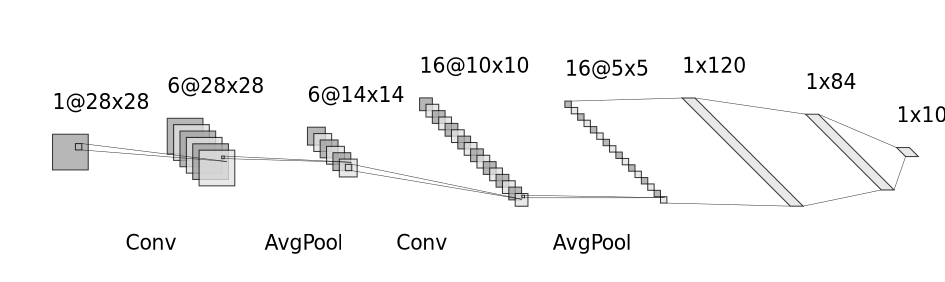
\includegraphics[scale=0.4]{midterm presentation/images/LeNet.png}
        \label{fig:lenet}
        \caption{LeNet network used for MNIST}
    \end{figure} 
\end{frame}

\begin{frame}{Cross-validation for Hyperparameter selection}
    We performed 4-Fold cross-validation on MNIST with LeNet:
    \begin{itemize}
        \item \textbf{Adam} : gridsearch for $\eta \in \{10^{-5}, 10^{-4}, 10^{-3}, 0.01, 0.1\}$ \newline
        Best value : $\eta = 10^{-4}$
        \item \textbf{SGD} : gridsearch for $\eta \in \{10^{-5}, 10^{-4}, 10^{-3}, 0.01, 0.1\}$ \newline
        Best value : $\eta = 0.1$
        \item \textbf{AdaGrad} : gridsearch for $\eta \in \{10^{-4}, 10^{-3}, 0.01, 0.1\}$ \newline
        Best value : $\eta = 0.1$
        \item \textbf{SVRG} : gridsearch for $\eta \in \{10^{-5}, 10^{-4}, 10^{-3}, 0.01, 0.1\}$ \newline
        Best value : $\eta = 0.01$
        \item \textbf{STORM} : gridsearch for $c \in \{10^{-5}, 10^{-4}, 10^{-3}, 0.01, 0.1\}$ and $k \in \{10^{-3}, 0.01, 0.1, 1\}$\newline
        Best value : $c = 100$ and $k=0.1$
        
    \end{itemize}
\end{frame}

\begin{frame}{Cross-validation example : Adam}
    \begin{figure}
        \centering
    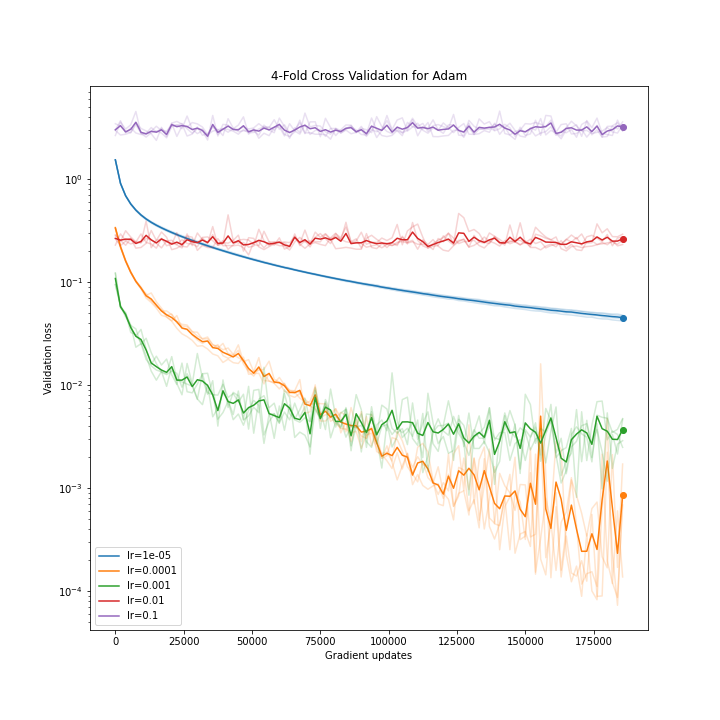
\includegraphics[scale=0.32]{midterm presentation/images/adamCV.png}
        \label{fig:adamCV}
    \end{figure}   
\end{frame}

\begin{frame}{Results on small Neural Network (LeNet)}
    \begin{figure}
        \centering
    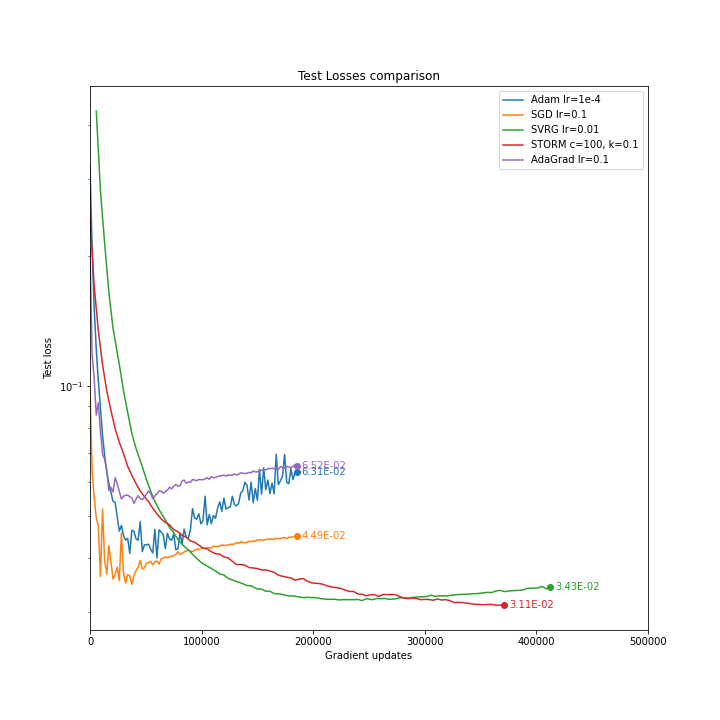
\includegraphics[scale=0.35]{midterm presentation/images/testLossesMnist.png}
        \label{fig:testLossesMnist}
    \end{figure}   
\end{frame}

\begin{frame}{Results on small Neural Network (LeNet)}

    We see that in this setup, \textbf{both variance reduced methods are performing better}.
    \newline
    It takes more time for SVRG and STORM to have better results. This is due in part to the two gradients that have to be computed per iteration and $\tilde{\mu}$ (the full gradient) that has to be computed every 5 iterations in SVRG.

\end{frame}

\begin{frame}{Variance reduced methods on deep neural networks}
    We want to test if variance reduced methods are still performing better on deep neural networks.
    \newline
    The paper "On the Ineffectiveness of Variance Reduced
    Optimization for Deep Learning"~\citep{Defazio2019} suggests that this is not the case, but:
    \begin{itemize}
        \item They give \textbf{no theoretical insights} why variance reduced methods perform poorly.
        \item They \textbf{use Batch-Norm Layers} in their setup. Batch-Norm layers break the assumption that the updates in SVRG are unbiased in expectation.
    \end{itemize}
\end{frame}

\begin{frame}{Our hypothesis}
    We want to check whether \textbf{removing Batch-Norm layers} and using other methods such as MetaInit can \textbf{help SVRG outperform} other algorithms as in the case of the setup with LeNet.
\end{frame}


\begin{frame}{Preliminary results on CIFAR10 with ResNet18}
    To test this hypothesis, we first use ResNet18 on the CIFAR10 dataset to see that in this setup (with BatchNorm layers) SVRG is outperformed.
    \begin{figure}
        \centering
    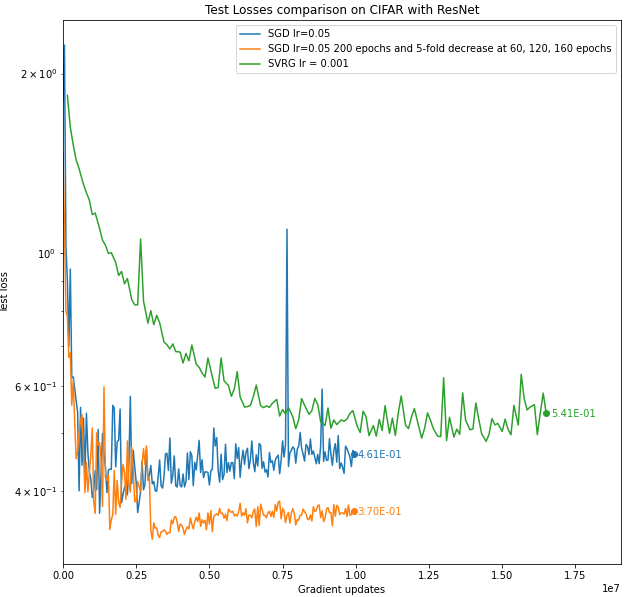
\includegraphics[scale=0.32]{midterm presentation/images/resnet18cifar.png}
        \label{fig:testLossesCifar}
    \end{figure}   
\end{frame}

\begin{frame}{Further steps}
    Plans for the rest of the project:
    \begin{itemize}
        \item Remove BatchNorm layers
        \item Compensate the effects of removed BatchNorm layers with \textbf{methods of initializing weights} 
        \begin{itemize}
            \item[] \textit{e.g.} MetaInit~\citep{dauphin2019metainit}
        \end{itemize}
        \item Apply the findings to a \textbf{deeper network} (ResNet50 ?)
    \end{itemize}
\end{frame}

\begin{frame}{ }
\begin{center}
    \Huge Thank you\\ Any questions?
\end{center}
   
\end{frame}


\begin{frame}[allowframebreaks]{References}
		\renewcommand*{\bibfont}{\tiny}
		\bibliography{main.bib}
   	% 	\bibliography{\jobname}
\end{frame}

\begin{frame}{MetaInit}
    Method for weights initialization introduced in 2019~\citep{dauphin2019metainit}.
    \begin{itemize}
        \item Deep Neural networks can be difficult to train, the performance depends heavily on how weights are initialized.
        \item Hypothesis of MetaInit: start training in regions tat look locally linear with minimal second order effects.
        \item MetaInit uses measures the above with a quantity called gradient quotient.
        \item The algorithm minimizes this quantity using GD to select the norms of initial weights.
    \end{itemize}
\end{frame}

\begin{frame}{ResNet}
    Network for image recognition introduced in 2015~\citep{he2015residual}.
    
    
\end{frame}

\end{document}

